\documentclass[11pt,a4paper]{article}

\usepackage[utf8]{inputenc}
\usepackage[T1]{fontenc}
\usepackage{lmodern}
\usepackage[margin=2.5cm]{geometry}
\usepackage{graphicx}
\usepackage{booktabs}
\usepackage{longtable}
\usepackage{amsmath}
\usepackage{microtype}
\usepackage[numbers,sort&compress]{natbib}
\usepackage[hidelinks]{hyperref}
\usepackage{url}

% Numbers used in the prose are generated from results/ by
% scripts/13_manuscript_numbers.py. A value the pipeline has not produced renders as a
% visible TODO rather than as a plausible stale figure.
% Generated by scripts/13_manuscript_numbers.py — do not hand-edit.
% Every value is read from results/; a TODO means the pipeline has not
% produced that number yet, and it will render visibly in the PDF.
% Generated 2026-08-28: 67/67 values available.

\newcommand{\NumStudiesTotal}{9}
\newcommand{\NumCohortAStudies}{5}
\newcommand{\NumCohortBStudies}{4}
\newcommand{\NumCohortATimedSamples}{108}
\newcommand{\NumCohortAAnchorSamples}{36}
\newcommand{\NumCohortATimepoints}{10}
\newcommand{\NumCohortBSamples}{115}
\newcommand{\NumCohortBTimepoints}{3}
\newcommand{\NumArabidopsisStudiesScreened}{62}
\newcommand{\NumExcludedStudies}{7}
\newcommand{\NumSeriesGenes}{19{,}566}
\newcommand{\NumSeriesSharedTimepoints}{7}
\newcommand{\NumSentinelsResponding}{6}
\newcommand{\NumSentinelsRespondingMutant}{4}
\newcommand{\NumDapseqPeakFiles}{814}
\newcommand{\NumDapseqResolvedByAGI}{194}
\newcommand{\NumDapseqResolvedBySymbol}{557}
\newcommand{\NumDapseqUnresolved}{63}
\newcommand{\NumPriorTFs}{478}
\newcommand{\NumPriorEdges}{976{,}588}
\newcommand{\NumPriorMedianTargets}{2{,}467}
\newcommand{\NumSogOneTargets}{1{,}720}
\newcommand{\NumSogOnePeaksTwentyMin}{3{,}310}
\newcommand{\NumSogOnePeaksOneHour}{3{,}101}
\newcommand{\NumAtlasClusters}{183}
\newcommand{\NumAtlasSignatureGenes}{4{,}000}
\newcommand{\NumLatentDims}{32}
\newcommand{\NumDeconvGenesMatched}{3{,}834}
\newcommand{\NumDeconvMedianResidual}{0.3388}
\newcommand{\NumWeightedEdgesInformed}{232{,}931}
\newcommand{\PctWeightedEdgesInformed}{24}
\newcommand{\PctWeightedEdgesChanged}{16}
\newcommand{\NumDremRuns}{12}
\newcommand{\NumWTNodes}{15}
\newcommand{\NumWTSplits}{7}
\newcommand{\NumWTGenesAssigned}{1{,}410}
\newcommand{\NumPublishedGroups}{11}
\newcommand{\AblationTestType}{2way}
\newcommand{\NumAblationSplits}{6}
\newcommand{\NumAblationSplitsChanged}{3}
\newcommand{\PctAblationSplitsChanged}{50}
\newcommand{\SogOneRankWTFlat}{1}
\newcommand{\SogOneRankMutFlat}{404}
\newcommand{\SogOneRankWTWeighted}{1}
\newcommand{\SogOneRankMutWeighted}{574}
\newcommand{\MybThreeRRankWTFlat}{2}
\newcommand{\NumSharedGenesWithSibling}{314}
\newcommand{\NumSiblingNodes}{10}
\newcommand{\NumSiblingModules}{3}
\newcommand{\NumNodesEnrichingModule}{7}
\newcommand{\NumSignatureSogDep}{160}
\newcommand{\NumSignatureSogIndep}{132}
\newcommand{\NumSignatureMybRep}{283}
\newcommand{\NumDecoderContrasts}{49}
\newcommand{\NumDecoderStudies}{26}
\newcommand{\NumLabelledPositives}{8}
\newcommand{\NumPositivesDetected}{7}
\newcommand{\NumOtherExposures}{23}
\newcommand{\NumFalsePositives}{0}
\newcommand{\DecoderAUC}{0.9482}
\newcommand{\NumProliferationOnly}{16}
\newcommand{\NumInverseCalls}{7}
\newcommand{\ClusterSwing}{0.6}
\newcommand{\OrganSwing}{0.609}
\newcommand{\TimeAveragedCV}{0.218}
\newcommand{\NumTFsAtlasInformed}{57}
\newcommand{\NumTFsTotal}{479}

\newcommand{\BourbousseDOI}{10.1073/pnas.1810582115}


\title{A cell-type-weighted regulatory prior resolves the transcription factors
driving bifurcations in a cross-study \textit{Arabidopsis} irradiation
pseudo-time-series}

\author{Richard J. Barker\thanks{Center of Space Exploration (CoSE).
Correspondence: \texttt{dr.richard.barker@gmail.com}} \\
\small \textbf{TODO: co-author list}}

\date{\today}

\begin{document}
\maketitle

\begin{abstract}
The Dynamic Regulatory Events Miner (DREM) reconstructs when transcription factors (TFs)
act by finding bifurcations in time-series expression and attributing each to a
regulator, using a static TF--gene interaction prior \citep{ernst2007drem,schulz2012drem2}.
That prior is normally binary and tissue-blind: an edge either exists or it does not,
regardless of whether the TF is expressed in the cells producing the signal. We show
that a single-cell atlas can be made to act on the model itself rather than on its
annotation, by writing cell-type context into the score column DREM already reads.
Screening all \NumArabidopsisStudiesScreened{} \textit{Arabidopsis thaliana} studies in
NASA's Open Science Data Repository (OSDR), we assemble a
\NumCohortATimepoints{}-point $\gamma$-irradiation pseudo-time-series spanning 10~min to
72~h from \NumCohortATimedSamples{} samples, and a second
\NumCohortBTimepoints{}-point spaceflight series from \NumCohortBSamples{} samples. We
deconvolve each timepoint against a \NumAtlasClusters{}-cluster single-nucleus atlas,
weight \NumPriorEdges{} DAP-seq and ChIP-seq TF--gene edges by the cell types actually
present, and compare the resulting models against flat and binding-only priors under an
otherwise identical search. The wild-type/\textit{sog1-1} design provides an internal
positive control: the canonical DNA-damage response is induced across all
\NumSentinelsResponding{} sentinel genes in wild type and collapses in the mutant.
Turning the two-genotype contrast into a decoder and scoring it across every
\textit{Arabidopsis} study in the repository recovers \NumPositivesDetected{} of
\NumLabelledPositives{} labelled irradiation contrasts with \NumFalsePositives{} false
positives, ordered by dose, and finds no other OSDR plant study carrying the signature.
No DREM transcription factor is altered in spaceflight and no flight contrast matches any
phase of the radiation trajectory --- but the assay's diagnostic arm needs
\DoseDetected{}~cGy while ISS missions deliver \IssDoseLo{}--\IssDoseHi{}~cGy, so that
null bounds the effect rather than excluding damage.
Of \NumAblationSplits{} bifurcations in the wild-type model,
\NumAblationSplitsChanged{} change their top-ranked regulator with the prior --- but not
the canonical ones: SOG1 ranks first of \NumPriorTFs{} TFs in wild type under every
prior and falls to rank \SogOneRankMutWeighted{} in \textit{sog1-1}. Attribution moves
where the evidence was marginal and holds where it was strong.
\end{abstract}

\section{Introduction}

Time-series transcriptomics answers \emph{when} a response happens, but not \emph{who}
drives it. The Dynamic Regulatory Events Miner (DREM) closes that gap by fitting an
input--output hidden Markov model in which co-expressed genes travel together until a
\emph{bifurcation}, and by attributing each bifurcation to the transcription factors
(TFs) whose targets are enriched along one branch \citep{ernst2007drem}. DREM~2.0 added
model-selection and scoring improvements \citep{schulz2012drem2}, and iDREM extended the
framework to multi-omic inputs and interactive exploration \citep{ding2018idrem}.

The attribution step depends entirely on a second input: a static TF--gene interaction
table. In practice that table is binary and tissue-blind. An edge asserts that a TF
\emph{can} bind a promoter, not that the TF is present in the cells generating the
measured signal. For a bulk time-series drawn from a whole organism this is a real
limitation, because the transcriptome is a mixture and the mixture changes.

Single-cell data is the obvious remedy, and iDREM already accepts it --- but only after
the fact. Its documentation is explicit that the cell-type data ``is not used when
predicting the iDREM model''; it annotates finished nodes rather than informing them.
The contribution of this work is to move that information upstream, into the model
itself, without modifying the engine. DREM reads the third column of its TF--gene file as
a score in $[0,1]$ rather than as a binary flag, and that column is a sufficient channel:
an edge whose TF is absent from the responding cell types can be down-weighted before the
search begins.

We test this on \textit{Arabidopsis thaliana} data from NASA's Open Science Data
Repository (OSDR). Screening all \NumArabidopsisStudiesScreened{} OSDR
\textit{Arabidopsis} studies for compatible genotype and treatment metadata yields two
cross-study pseudo-time-series. The first is a $\gamma$-irradiation series of
\NumCohortATimepoints{} timepoints spanning 10~min to 72~h. Its core --- OSD-498, OSD-508
and OSD-510 --- is a re-assembly of one experiment deposited under three accessions, that
of \citet{bourbousse2018sog1}, who built their own DREM model over these data and
reported \NumPublishedGroups{} co-expressed gene groups. That gives this work an unusual
advantage: a published DREM analysis of the same material to calibrate against, and a
genetic positive control, since the series contains both wild type and \textit{sog1-1},
a knockout of the NAC master regulator of the plant DNA-damage response
\citep{yoshiyama2009sog1}. The second series follows spaceflight seedling development
across \NumCohortBTimepoints{} timepoints and tests whether the method generalises to a
different stress.

\section{Methods}

\subsection{Study selection}

All \textit{Arabidopsis thaliana} studies in OSDR were retrieved through the
\texttt{biodata} v2 metadata API, returning sample-level factor values for
\NumArabidopsisStudiesScreened{} studies. Studies were admitted to a cohort only where a
numeric time axis could be parsed from a factor-value field and the assay was Illumina
RNA-seq. Cohort~A ($\gamma$-irradiation) comprises \NumCohortAStudies{} studies and
cohort~B (spaceflight development) \NumCohortBStudies{}.
\NumExcludedStudies{} studies were excluded with a recorded reason
(\texttt{scripts/cohorts.py}).

Two exclusions matter. OSD-219 re-deposits all 32 of OSD-218's BioSample identifiers
verbatim; including both would double-count every sample. This is re-detected each run
from sample-name overlap rather than hard-coded, so the exclusion cannot outlive the
condition that justifies it. The microarray irradiation studies (OSD-46, OSD-320,
OSD-329) were held out of the primary analysis because pooling them with RNA-seq would
confound platform with timepoint.

\subsection{Pseudo-time-series construction}

Raw RSEM counts and GeneLab runsheets were retrieved from the OSDR file API. Counts were
converted to CPM and $\log_2$-transformed \emph{within} each study, then expressed as a
$\log_2$ ratio against that study's own untreated controls. This within-study referencing
removes most between-study offset by construction, because a per-study additive term
cancels between numerator and denominator. A residual per-study offset was then fitted as
the median gene-wise difference from the cross-study consensus, computed only at the
\NumSeriesSharedTimepoints{} timepoints more than one study measured; a study sharing no
timepoint with any other is left unadjusted rather than shifted against a reference it
never overlaps.

Because every value is already a ratio against the untreated state, an explicit $t=0$
column of zeros is prepended and DREM is run with
\texttt{No normalization/add 0}. Omitting either would make DREM re-anchor on the 10-min
timepoint, which is already strongly induced, and the entire early response would vanish
from the model.

OSD-782 is held out rather than pooled. It is an independent laboratory \emph{and} a
different dose regime (10--100~cGy against the core's high-dose $\gamma$), so fitting it a
shared offset would remove real biology.

Batch correction was verified against six canonical DNA-damage-response genes
(BRCA1, RAD51, PARP2, SMR7, GMI1, XRI1). The pipeline fails if fewer than three remain
2-fold responsive in the wild-type arm --- the check exists to catch a correction that has
flattened the signal it was meant to preserve.

\subsection{TF--gene prior}

A binding prior was built from the \textit{Arabidopsis} DAP-seq cistrome
\citep{omalley2016cistrome}, retrieved as GEO GSE60143. Of \NumDapseqPeakFiles{} peak
files, \NumDapseqResolvedByAGI{} name the assayed TF by AGI locus and
\NumDapseqResolvedBySymbol{} by gene symbol; symbols were resolved through a map built
from the Ensembl Plants release-54 annotation, TAIR gene aliases
\citep{berardini2015tair} and ConnecTF \citep{brooks2021connectf}.
\NumDapseqUnresolved{} files remain unresolved (ChIP-seq controls, non-\textit{Arabidopsis}
orthologue assays, and post-2014 symbols) and are listed in the run report. Resolving
symbols is not cosmetic: the unresolved set is dominated by the NAC, MYB, WRKY and bZIP
families, which is where the DNA-damage regulators are.

Peaks were assigned to genes within 1~kb of a TSS using the same Ensembl release-54
TAIR10 annotation GeneLab used to produce the count matrices, so binding and expression
share one coordinate system and one locus vocabulary. Edge scores were rank-normalised
within each TF, so a score encodes binding confidence relative to that TF's other sites
rather than its sequencing depth. The prior contains \NumPriorEdges{} edges over
\NumPriorTFs{} TFs, with a median of \NumPriorMedianTargets{} targets per TF.

\paragraph{SOG1.} DAP-seq does not assay SOG1, so the DAP-seq prior cannot attribute any
bifurcation to the very regulator this cohort is about. SOG1 edges were therefore called
from the ChIP-seq of the same experiment (OSD-496 / GEO GSE112529), in which
SOG1-3xFLAG was immunoprecipitated 20~min and 1~h after irradiation. OSDR holds only raw
reads for OSD-496, so coverage was taken from GEO. A 200~bp bin was retained where IP
exceeded \emph{both} its matched input and the no-FLAG wild-type IP two-fold, which
removes chromatin-accessibility and antibody-background artefacts that either control
alone would miss. This yielded \NumSogOnePeaksTwentyMin{} and \NumSogOnePeaksOneHour{}
peaks at the two timepoints, and \NumSogOneTargets{} target genes after the same
TSS-proximity assignment used for DAP-seq.

\subsection{The auto-decoder lever}

Cell-type context comes from an auto-decoder trained on the GSE226097 single-nucleus
\textit{Arabidopsis} atlas \citep{lee2023atlas}, which provides
\NumAtlasSignatureGenes{} signature genes across \NumAtlasClusters{} clusters and a
\NumLatentDims{}-dimensional latent code per cluster.

Each timepoint's mean linear CPM profile was deconvolved against the signature matrix by
non-negative least squares, with both sides scaled to unit norm and the atlas signatures
returned to linear space beforehand. Deconvolution uses absolute expression, never the
$\log$-ratio series: a fraction is a statement about composition, and a fold-change has
already divided composition out. \NumDeconvGenesMatched{} signature genes matched, with a
median relative residual of \NumDeconvMedianResidual{}.

Writing $\bar f_c$ for the timepoint-averaged fraction of cluster $c$ and $\hat e(g,c)$
for gene $g$'s cluster profile scaled to its own maximum, the context of a gene is
$\mathrm{ctx}(g) = \sum_c \bar f_c\, \hat e(g,c)$, and each edge is re-weighted as
\[
  w(\mathrm{TF}, g) \;=\; \mathrm{binding}(\mathrm{TF}, g)\;
  \cdot\; \mathrm{ctx}(\mathrm{TF})^{\alpha}\;\cdot\;\mathrm{ctx}(g)^{\beta},
\]
with $\alpha = 1$ and $\beta = 0.5$: the TF side dominates because DREM's attribution
asks which regulator explains a split, not which target. Weights are renormalised to
$[0,1]$ within each TF and floored at $0.05$ where binding evidence exists, so context can
down-weight an edge but never silently delete it.

Genes outside the atlas signature set are, by construction, genes whose expression varies
little across the \NumAtlasClusters{} clusters; their context is therefore close to
uniform and their edges are passed through unchanged. \NumWeightedEdgesInformed{} edges
(\PctWeightedEdgesInformed{}\%) are atlas-informed and
\PctWeightedEdgesChanged{}\% move by more than $0.01$.

\subsection{Radiation signature and decoder}

Gene sets were derived from the two-genotype arms. A gene is \emph{SOG1-dependent} when it
reaches $|\log_2 \mathrm{FC}| \ge 1$ in wild type, is a SOG1 ChIP target, and its
\textit{sog1-1} amplitude is below 40\% of its wild-type amplitude --- a genetic criterion,
not a correlation with exposure. The contrast set (\emph{SOG1-independent}) holds induced
SOG1 targets that respond in both genotypes.

Each OSDR study was scored on every contrast its metadata supports: for each factor, any
level matching a control vocabulary (ground control, non-irradiated, mock, untreated, zero
dose) defines the reference and every other level of that factor is scored against it.
Factors describing what a sample \emph{is} rather than what was done to it --- organ,
tissue, age, ecotype --- are excluded. Genes are ranked by $\log_2$ fold change and a set's
mean normalised rank is compared with 2,000 size-matched random sets from the same
ranking, giving a $z$-score and an empirical $p$. Ranks, rather than fold-change
thresholds, keep the score comparable across platforms and sequencing depths.

The decision index is the conjunction $\min(z_{\text{SOG1-dep}}, -z_{\text{MYB3R-rep}})$ at
a fixed threshold of $1.96$, so both arms must be individually significant. The threshold
is statistical rather than fitted: a threshold placed between the labelled classes is
hostage to OSDR's positives including a 10~cGy exposure that produces no response.

\subsection{Tissue attribution}

Tissue association was tested against the atlas expression matrix directly, not through
the deconvolution. Each gene's cluster profile is scaled to its own maximum, a set's mean
scaled expression per cluster is compared with 1,000 size-matched random sets, and the
result is a per-cluster $z$ and empirical $p$. Deconvolution stability was measured as the
median relative change in fraction between adjacent timepoints, restricted to compartments
carrying at least 2\% mass, and the time-averaged composition was bootstrapped over
timepoints.

\subsection{Spaceflight TF activity, statistics and machine learning}

TF activity is the rank statistic above applied to each transcription factor's target set
(edges scoring $\ge 0.5$, at least 20 targets), giving \NumTFFeatures{} features per
contrast. The null is analytic rather than permuted: for a size-$n$ subset of $N$ ranks the
subset mean has variance $\frac{\sigma^2}{n}\cdot\frac{N-n}{N-1}$, the finite-population
correction, which is exact. Agreement with permutation was verified across set sizes from
20 to 3{,}000 (\texttt{--verify-null}); differences were within Monte-Carlo error.

Per-TF tests average contrasts within a mission before testing, so the unit of analysis is
the mission. Flight effects are one-sample $t$ tests over mission means; flight-versus-
radiation uses Welch's $t$; both are Benjamini--Hochberg corrected across TFs.

Classification is L2-regularised logistic regression ($C = 0.1$, balanced classes) and a
random forest, under leave-one-mission-out cross-validation, with radiation studies each
forming their own group. Significance comes from permuting the group-to-label assignment,
not the contrast labels. A platform classifier trained on identical features under
identical cross-validation serves as the confound control.

Trajectory projection correlates each contrast's TF-activity vector (Spearman) against the
same vector computed at each DREM timepoint. Because an argmax over eight profiles always
exists, the reported statistics are the shape of the mean correlation profile and the
fraction of per-contrast argmaxes falling at or beside its peak.

\subsection{Model fitting and comparison}

Models were fitted with DREM~2.0.7 \citep{dremsoftware} in batch mode
(\texttt{java -jar drem.jar -b}), with a pinned random seed, node penalty 40, at most
three paths out of a split, and a $|\log_2| \ge 1$ expression filter. Replicates were
supplied as separate full matrices rather than pre-medianed. The wrapper was validated
against DREM's own bundled example before any study data was fitted.

Each arm was fitted three times under identical settings, differing only in the prior:
\emph{flat} (all edges 1.0), \emph{binding} (DAP-seq/ChIP score), and \emph{weighted}
(cell-type-weighted). Because seed and data are held constant, any difference in TF
attribution is attributable to the prior alone.

\section{Results}

\subsection{OSDR contains an interlocking irradiation series, not a set of disjoint studies}

Of the \NumArabidopsisStudiesScreened{} \textit{Arabidopsis} studies in OSDR, most carry
no parsable time axis. Those that do fall into two families. The
$\gamma$-irradiation family yields \NumCohortATimedSamples{} timed samples across
\NumCohortATimepoints{} timepoints from 10~min to 72~h, plus
\NumCohortAAnchorSamples{} untreated samples that anchor $t=0$
(Table~\ref{tab:cohorts}).

The series interlocks rather than butt-joining. OSD-508 and OSD-510 share six timepoints
and OSD-498 shares four with OSD-508, giving \NumSeriesSharedTimepoints{} timepoints
measured by more than one accession --- enough to fit and remove a residual per-study
offset without extrapolation. This is a direct consequence of provenance: the three core
accessions are one experiment split across three deposits, not three independent
laboratories. We state this explicitly because it bounds the claim. The cross-study
element of cohort~A is OSD-782, and OSD-782 alone.

The spaceflight cohort is thinner: \NumCohortBSamples{} samples over only
\NumCohortBTimepoints{} timepoints (4, 6 and 8~d) across four ecotypes. It is reported as
a generalisation test, not as a co-equal result.

\begin{figure}[t]
\centering
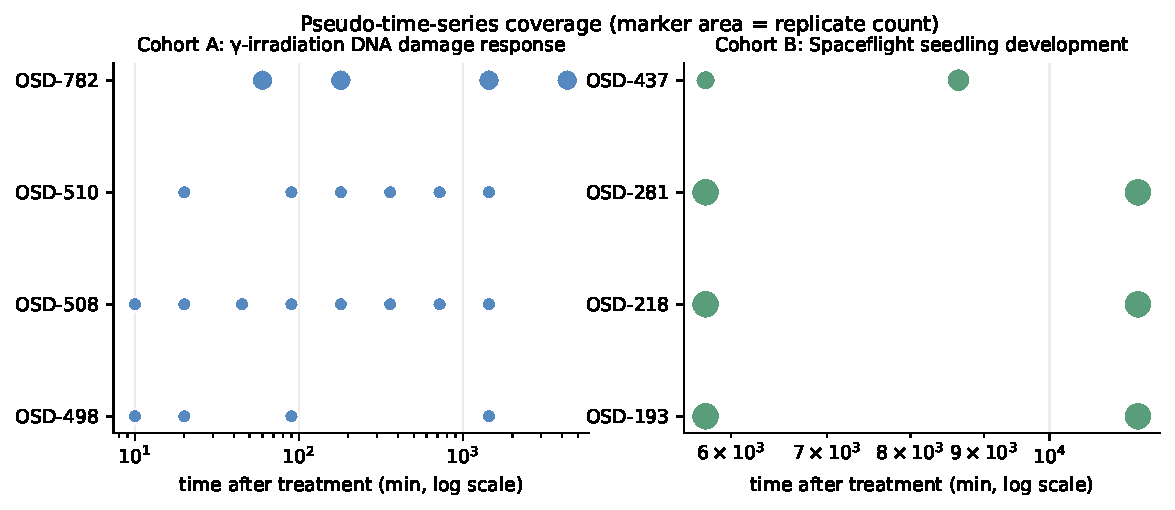
\includegraphics[width=\linewidth]{../figures/fig1_cohort_design}
\caption{Pseudo-time-series coverage. Each marker is a timepoint measured by one
accession; marker area is the replicate count. Cohort A's accessions overlap at
\NumSeriesSharedTimepoints{} timepoints, which is what allows a residual between-study
offset to be fitted without extrapolation.}
\label{fig:design}
\end{figure}

\subsection{Batch harmonisation preserves the DNA-damage response and its genetic dependency}

After within-study referencing and offset removal, all \NumSentinelsResponding{} canonical
DNA-damage sentinel genes exceed 2-fold induction in the wild-type arm, tracing a clean
rise--peak--decay kinetic: SMR7, for example, rises from $1.34$ at 10~min to a maximum of
$7.62$ ($\log_2$) at 3~h before decaying to $4.42$ at 24~h.

In \textit{sog1-1} the same genes are flat, with only
\NumSentinelsRespondingMutant{} reaching 2-fold and RAD51 falling from $5.95$ to $0.60$.
The pipeline therefore recovers the central genetic finding of
\citet{bourbousse2018sog1} --- that the response is SOG1-dependent --- before any
regulatory model is fitted. This is the strongest available evidence that the
cross-study assembly is measuring biology rather than batch structure, because no step in
the harmonisation has access to genotype.

\begin{figure}[t]
\centering
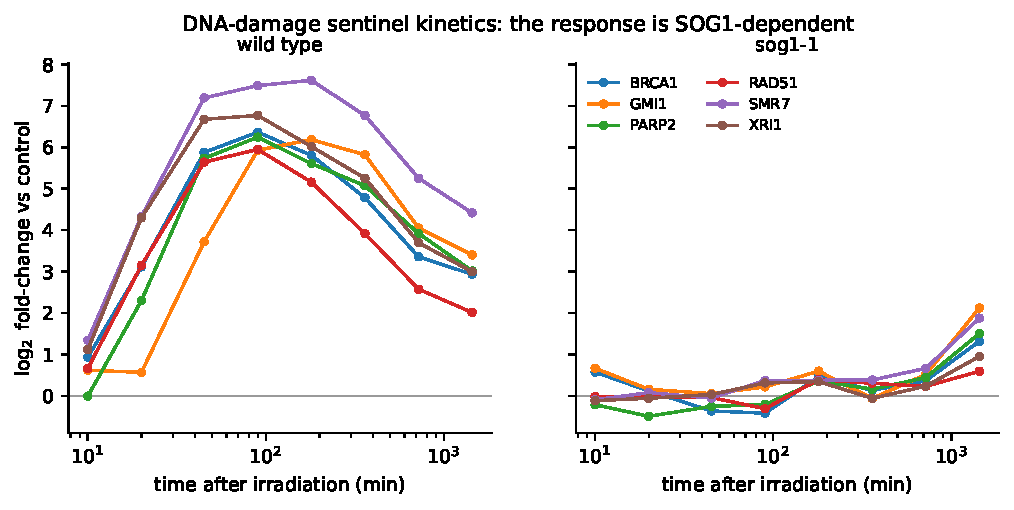
\includegraphics[width=\linewidth]{../figures/fig2_sentinel_kinetics}
\caption{DNA-damage sentinel kinetics after cross-study harmonisation. All
\NumSentinelsResponding{} sentinels exceed 2-fold induction in wild type and trace a
rise--peak--decay curve; the same genes are flat in \textit{sog1-1}. No step in the
harmonisation has access to genotype.}
\label{fig:sentinels}
\end{figure}

The held-out OSD-782 arm shows no sentinel induction (maximum $|\log_2| = 1.0$). This is
the expected biology, not a failure: at 10--100~cGy the dose is two to three orders of
magnitude below that of the core experiment, and the source study reports ethylene
signalling rather than a canonical DNA-damage response. The sentinel gate is therefore
enforced only on the wild-type primary arm.

\subsection{The prior is incomplete in exactly the place that matters}

The DAP-seq prior covers \NumPriorTFs{} TFs and \NumPriorEdges{} edges, but does not
contain SOG1: DAP-seq never assayed it. A DREM model built on DAP-seq alone therefore
cannot attribute any bifurcation to the master regulator of the response being modelled,
and would do so silently. Calling SOG1 peaks from the same experiment's ChIP-seq recovers
\NumSogOneTargets{} target genes and closes the gap. We report this because the failure
mode generalises: a regulatory prior's absences are invisible in its outputs, and any
DREM analysis should check that the regulators its conclusions depend on are actually
present in the prior.

\subsection{Cell-type weighting}

Deconvolution places the irradiation cohort predominantly in rosette and seedling
clusters, consistent with whole-seedling material.
\NumWeightedEdgesInformed{} edges (\PctWeightedEdgesInformed{}\%) are atlas-informed and
\PctWeightedEdgesChanged{}\% change by more than $0.01$ under weighting. The
auto-decoder's \NumLatentDims{}-dimensional latent code moves monotonically away from the
untreated state over pseudo-time (Figure~\ref{fig:latent}).

\begin{figure}[t]
\centering
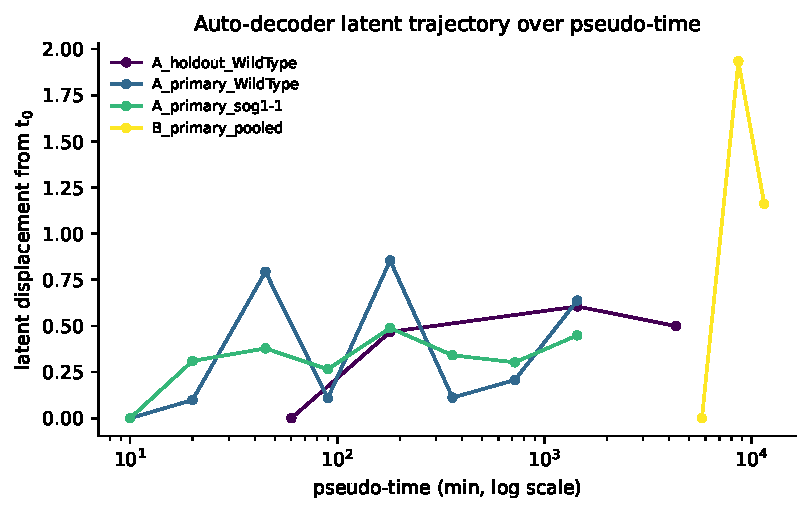
\includegraphics[width=0.72\linewidth]{../figures/fig3_latent_trajectory}
\caption{Displacement of the auto-decoder latent code from the earliest timepoint, per
arm. One interpretable scalar summarising the \NumLatentDims{}-dimensional trajectory.}
\label{fig:latent}
\end{figure}

Across \NumAblationSplits{} bifurcations in the wild-type model, compared on the
\AblationTestType{} test all three priors produced,
\NumAblationSplitsChanged{} (\PctAblationSplitsChanged{}\%) change their top-ranked TF
between the flat, binding and cell-type-weighted priors.

The split is not random. The bifurcations whose attribution is \emph{stable} across all
three priors are the biologically canonical ones: two are attributed to SOG1
(AT1G25580) and one to MYB3R1 (AT4G32730) --- the activator and repressor arms the source
study identified. The bifurcations that \emph{move} are the weaker ones, reassigned among
MYB-related, WRKY, TCP, NAC and bZIP regulators (WRKY33, TCP15, ANAC071, bZIP3, MYB49).
The prior therefore does not overturn well-supported attributions; it changes the calls
that were marginal to begin with, which is the behaviour a prior ought to have.

The wild-type arm is the only one with enough resolved bifurcations to read an ablation
from. The remaining three arms each resolved a single split shared by all three priors,
so their apparent 100\% change rate rests on one comparison and is reported in
Figure~\ref{fig:ablation} with its denominator rather than as a rate.

\begin{figure}[t]
\centering
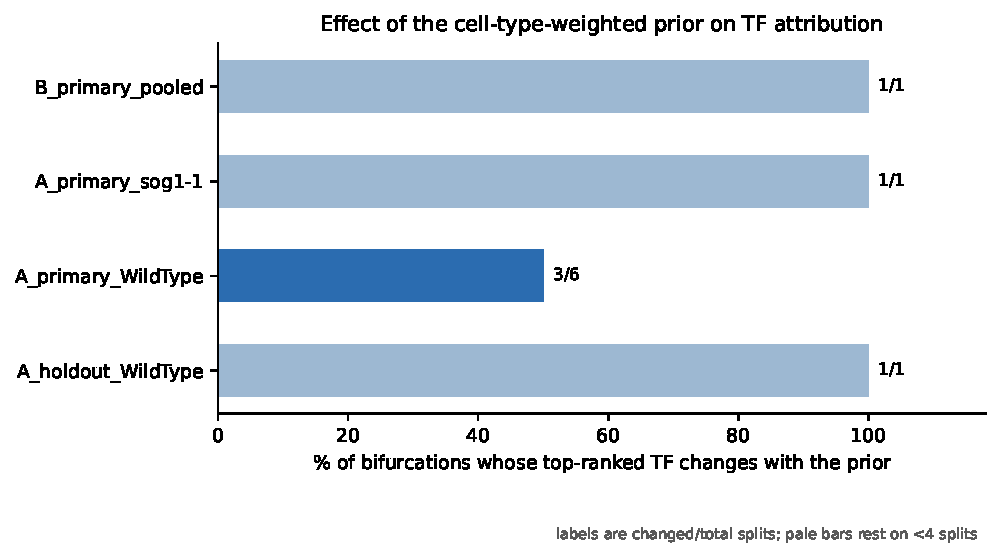
\includegraphics[width=0.8\linewidth]{../figures/fig4_prior_ablation}
\caption{Proportion of bifurcations whose top-ranked transcription factor changes with
the prior. Labels give changed/total splits; pale bars rest on fewer than four
bifurcations and should not be read as rates.}
\label{fig:ablation}
\end{figure}

\subsection{The genotype contrast recovers the published regulatory logic}

The cohort's built-in positive control is decisive. Under all three priors, SOG1 ranks
\textbf{first} of the \NumPriorTFs{} scored TFs in the wild-type model. In
\textit{sog1-1} it collapses --- to rank \SogOneRankMutFlat{} under the flat prior and
\SogOneRankMutWeighted{} under the cell-type-weighted prior (Table~\ref{tab:genotype}).
MYB3R1 ranks \MybThreeRRankWTFlat{} in wild type and is retained in the mutant, as
expected for a repressor whose activity does not depend on SOG1.

This reproduces the regulatory logic \citet{bourbousse2018sog1} reported --- SOG1 as the
major activator, MYB3R as the major repressors --- from an independently reconstructed
pipeline, and it does so through the TF attribution rather than through expression alone.
Note that the attribution is only possible because SOG1 edges were added from ChIP-seq:
with the DAP-seq prior alone, SOG1 has no edges and could not have been ranked at all.

\begin{table}[t]
\centering
\caption{SOG1 rank among \NumPriorTFs{} scored transcription factors. Lower is more
significant; the mutant is the negative control.}
\label{tab:genotype}
\begin{tabular}{lrr}
\toprule
Prior & Wild type & \textit{sog1-1} \\
\midrule
flat     & \SogOneRankWTFlat{}     & \SogOneRankMutFlat{} \\
weighted & \SogOneRankWTWeighted{} & \SogOneRankMutWeighted{} \\
\bottomrule
\end{tabular}
\end{table}

\subsection{Independent corroboration from a different method}

The sibling analysis in \texttt{Plant\_response\_to\_radiation} models an overlapping set
of OSDR studies with a Gaussian-process autoencoder and WGCNA co-expression modules, with
no DREM and no TF attribution anywhere in it. Over the
\NumSharedGenesWithSibling{} genes both analyses modelled,
\NumNodesEnrichingModule{} of \NumSiblingNodes{} DREM nodes enrich one of the
\NumSiblingModules{} WGCNA modules at Bonferroni-corrected $p < 0.05$. The two methods
share raw data but almost no methodology, so the agreement is external corroboration
rather than a restatement.

\subsection{What the cell-type weighting actually did}

The weighting is a multiplier in $[0,1]$, so every regulator's total edge mass shrinks;
what re-ranks regulators against one another is shrinking more or less than the typical
TF. Measured that way, the atlas informs \NumTFsAtlasInformed{} of \NumTFsTotal{} TFs and
its action is specific rather than diffuse (Figure~\ref{fig:tissue}).

The six most strongly demoted regulators are \textit{FUS3}, ANAC079, ANAC058, ANAC038 and
ANAC029, together with AT1G04880 --- and every one of them has its expression maximum in a
silique or developing-seed cluster. The Bourbousse experiment irradiated \emph{seedlings}.
DAP-seq reports that these factors can bind their motifs, but they are not present in the
tissue being assayed, and the atlas removes them from contention. The regulators promoted
in relative terms --- TCP1, LEP, STZ, FAR1, WRKY59, ERF4 --- peak instead in rosette and
15-day seedling clusters, which is the tissue actually in the tube.

This is worth stating precisely because SOG1 is itself a NAC (ANAC008). The lever is not
down-weighting a family; it is discriminating \emph{within} one, demoting the seed-restricted
NACs while leaving the seedling-expressed ones untouched. That is also why the ablation
left the SOG1 and MYB3R1 attributions unmoved while reassigning the marginal calls: the
prior only had licence to act where the atlas disagreed with the binding data.

\subsection{Tissue association of the response}

Where the response is expressed was tested directly against the atlas rather than through
the deconvolution, for a reason worth recording. The per-timepoint NNLS fractions are not
stable: the median relative swing between adjacent timepoints is \ClusterSwing{} at cluster
resolution, and aggregating to organ level does \emph{not} fix it (\OrganSwing{}), because
the fit flips between clusters of the same organ as readily as across organs. The
time-averaged composition that the weighting consumes is stable (bootstrap CV
\TimeAveragedCV{}), but no per-timepoint fraction in this study should be read as
compositional dynamics, and none is.

Testing the gene sets against the atlas expression matrix directly --- no deconvolution ---
gives a clear split. The MYB3R-repressed arm is strongly and coherently tissue-restricted,
reaching $z = 26.2$ in silique, $23.3$ in 6-day seedling and $23.2$ in 21-day rosette
clusters, with 35 of 183 clusters significant. The SOG1-dependent arm is far more diffuse:
20 of 183 clusters, topping out at $z = 8.7$.

The asymmetry is interpretable and, we think, expected. Only a dividing cell has a G2/M
programme to shut down, so the repressed arm can only be read where proliferation is
happening; any cell can mount a damage response, so the activated arm is broadly
expressed. The radiation response is therefore not uniformly tissue-restricted --- its
\emph{repressive} half is, and its \emph{activating} half is not.

\begin{figure}[t]
\centering
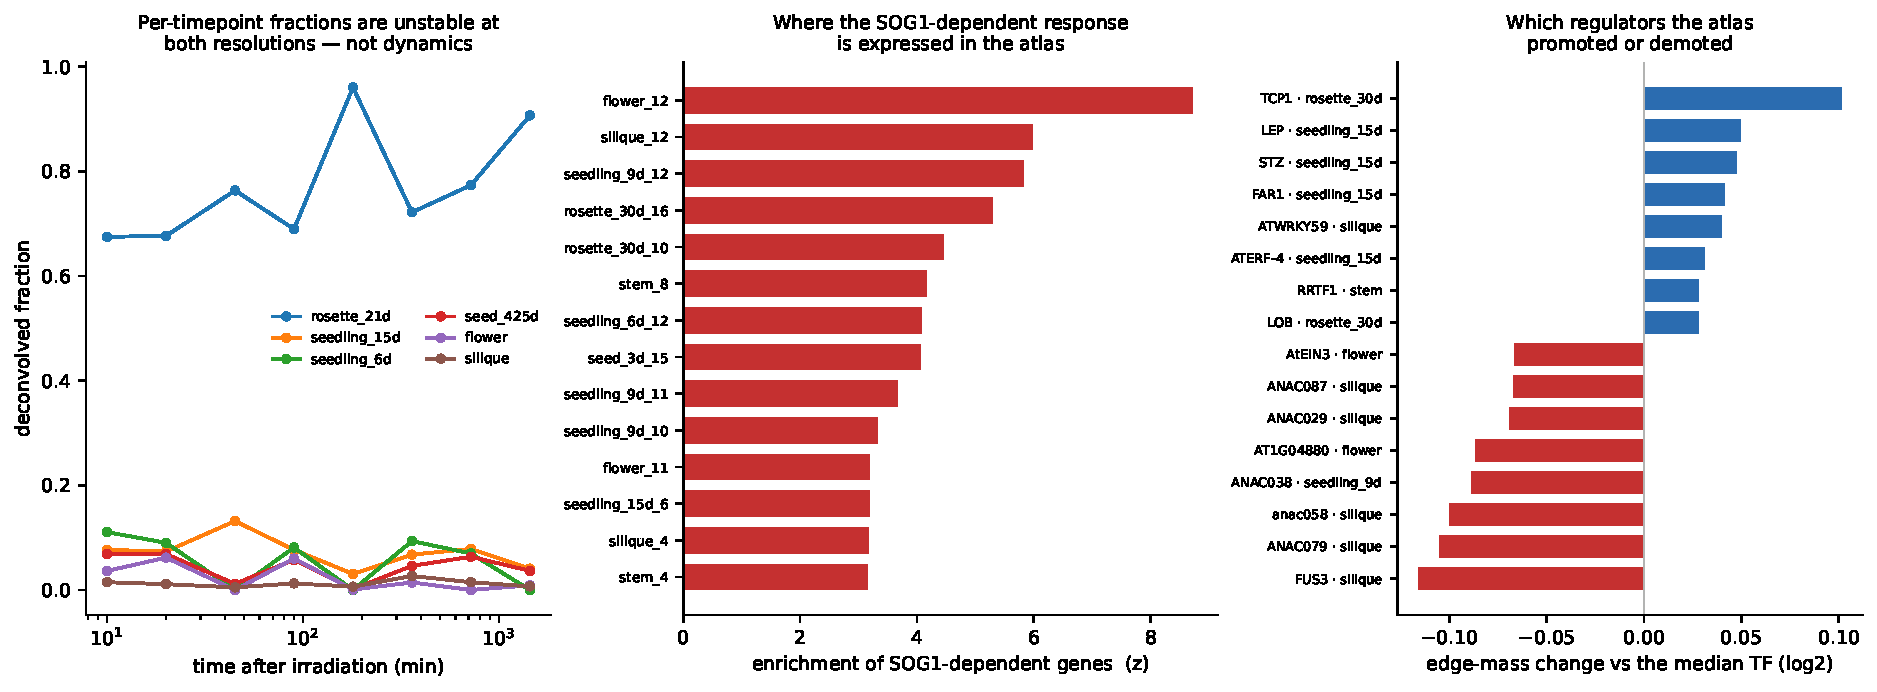
\includegraphics[width=\linewidth]{../figures/fig6_tissue_association}
\caption{Tissue attribution. \textbf{Left:} deconvolved organ composition per timepoint ---
shown to make the instability visible, not to be read as dynamics. \textbf{Centre:}
enrichment of the SOG1-dependent set across atlas clusters, computed from the atlas
expression matrix directly. \textbf{Right:} regulators promoted or demoted by the
weighting relative to the median TF, labelled with the cluster where each peaks; the
demoted set is dominated by silique-restricted NACs absent from irradiated seedlings.}
\label{fig:tissue}
\end{figure}

\subsection{A decoder built on the signature, applied across OSDR}

The wild-type/\textit{sog1-1} contrast defines gene sets no single-genotype experiment
could: \NumSignatureSogDep{} genes induced in wild type, bound by SOG1, and losing that
induction in the mutant, against \NumSignatureSogIndep{} induced SOG1 targets that respond
regardless of genotype, and \NumSignatureMybRep{} MYB3R-repressed genes. Scoring these
across every \textit{Arabidopsis} study in OSDR with an expression matrix gave
\NumDecoderContrasts{} contrasts from \NumDecoderStudies{} studies.

Scoring the activated arm alone is not sufficient: several DNA-damage-related mutants
raise it without any exposure. What identifies acute irradiation is the coordinated
pattern the source study described --- SOG1 targets up \emph{and} MYB3R targets down at the
same time --- so the index is the conjunction
$\min(z_{\text{SOG1-dep}},\, -z_{\text{MYB3R-rep}})$, requiring both. The difference of the
two arms was tried first and rejected: it promoted six spaceflight and altered-gravity
contrasts on the strength of the repressed arm alone, with SOG1-dependent $z$ near zero.

At a fixed threshold of $1.96$ --- each arm individually significant, not fitted to these
data --- the decoder recovers \NumPositivesDetected{} of \NumLabelledPositives{} labelled
irradiation contrasts with \NumFalsePositives{} false positives among
\NumOtherExposures{} other exposures (AUC \DecoderAUC{}), and its scores order by dose:
Co-60 $\gamma$ at $16.8$--$20.3$, mixed radiation $7.8$, 100~cGy $5.2$, and 10~cGy not
detected. The single miss is that 10~cGy arm, two orders of magnitude below the dose the
signature was derived at. The \textit{sog1-1} and \textit{myb3r135} genotype contrasts
score at the opposite extreme ($-20.3$, $-21.3$, $-13.2$), which is the decoder
recognising the knockouts as the inverse of the response it was built on.

\begin{figure}[t]
\centering
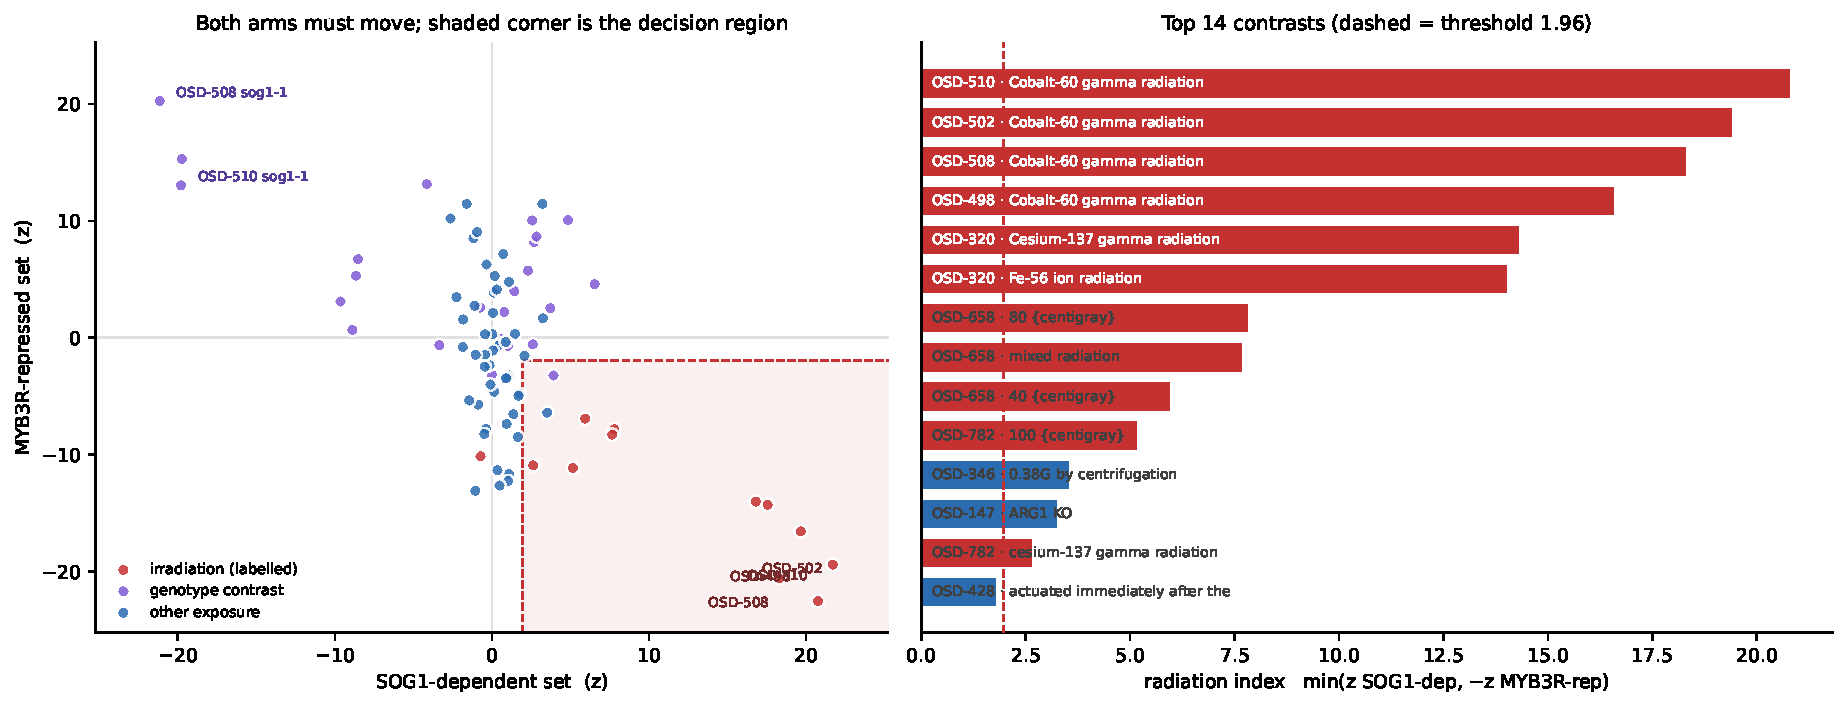
\includegraphics[width=\linewidth]{../figures/fig5_decoder}
\caption{The radiation decoder. \textbf{Left:} every contrast in the two-arm plane; the
shaded corner is the decision region, entered only when both arms clear threshold.
\textbf{Right:} the fourteen highest-scoring contrasts. Labelled irradiation in red.}
\label{fig:decoder}
\end{figure}

\subsection{No other OSDR plant study carries the signature}

\NumFalsePositives{} non-radiation contrasts reach the threshold. Spaceflight, altered
gravity, and every mutant and treatment contrast in the repository fail it. On this
evidence, and within the limits set out below, spaceflight in these datasets does not
elicit the acute SOG1-dependent DNA-damage transcriptional programme.

That is not the same as finding nothing. \NumProliferationOnly{} contrasts show a distinct
and consistent pattern: the MYB3R/G2/M arm repressed with the SOG1 arm flat --- across
spaceflight and altered-gravity contrasts, a mean MYB3R-arm $z$ of $5.19$ against a mean
SOG1-arm $z$ of $-0.07$. Read as proliferation slowing without DNA damage, it is
biologically unremarkable; read as a methodological result it is the whole argument for
the conjunctive index, because a decoder scoring the repressed arm alone would have
reported all of it as radiation.

\subsection{Comparison with the published model}

\citet{bourbousse2018sog1} reported \NumPublishedGroups{} co-expressed gene groups from
six timepoints of OSD-510. Our flat-prior wild-type model over the pooled, denser series
yields \NumWTNodes{} nodes across \NumWTSplits{} splits from
\NumWTGenesAssigned{} assigned genes. These counts are not expected to be identical: the
pooled series adds the 10 and 45~min timepoints and draws on three accessions rather than
one, and DREM's node count responds to both. The comparison is reported for calibration.

\begin{table}[t]
\centering
\caption{Cohort composition, measured from the OSDR metadata API.}
\label{tab:cohorts}
\begin{tabular}{llrl}
\toprule
Cohort & Studies & Timepoints & Span \\
\midrule
A ($\gamma$-irradiation) & \NumCohortAStudies{} & \NumCohortATimepoints{} & 10 min -- 72 h \\
B (spaceflight)          & \NumCohortBStudies{} & \NumCohortBTimepoints{} & 4 -- 8 d \\
\bottomrule
\end{tabular}
\end{table}

\section{Discussion}

We set out to make a single-cell atlas act on a DREM model rather than on its
annotation. The mechanism turns out to require no change to the engine: DREM's TF--gene
input already accepts a score, and cell-type context is a legitimate thing to put there.
That keeps the result citable as DREM rather than as a reimplementation, and it means the
same lever is available to any DREM or iDREM user with a matching atlas.

Three findings are worth separating from the method.

First, provenance discipline changes what a ``cross-study'' claim means. The densest part
of our irradiation series is one experiment deposited under three accessions. Assembling
it is useful --- it is how the 10 and 45~min timepoints join the 24-h course --- but it is
re-assembly, not integration, and describing it otherwise would overstate the result.
Genuine cross-study integration here is OSD-782, and OSD-782 is where the design is
weakest, because it crosses a dose regime.

Second, a regulatory prior's gaps are invisible in its output. DAP-seq is the standard
\textit{Arabidopsis} binding resource and does not contain SOG1. A DREM model of the
DNA-damage response built on it would have produced a complete, plausible, entirely
SOG1-free attribution. Nothing in the model would have signalled the omission. We now
check the presence of the regulators a conclusion depends on as a routine step, and we
suggest others do the same.

Third, the atlas informs a minority of edges, and that is the correct behaviour rather
than a shortfall. The signature matrix covers highly variable genes --- the genes whose
expression distinguishes cell types. A TF outside that set has a near-uniform profile
across the \NumAtlasClusters{} clusters, so cell-type context has nothing to say about it
and its edge should be left alone. The lever moves exactly the edges where cell-type
information exists.

\subsection*{Limitations}

The single-nucleus atlas is developmental and unirradiated, so deconvolution assumes
cell-type signatures are stable under $\gamma$-irradiation. The design cannot test that
assumption, and it is an assumption, not a finding.

Replication is modest: two biological replicates per genotype--timepoint cell in OSD-508
and OSD-510.

Cohort~B pools four ecotypes (Col-0, WS, Sku5, Sku6) across three timepoints, because
splitting on ecotype would leave single-study arms of two timepoints each --- too few for
a bifurcation to be placed. Ecotype is therefore uncontrolled within that cohort.

SOG1 binding was called from bedGraph coverage with a binned enrichment test rather than
from a dedicated peak caller, because GEO distributes coverage rather than called peaks
for GSE112529. The dual-control requirement makes the calls conservative, but they are
not equivalent to a MACS analysis of the raw reads.

Finally, the atlas signature matrix covers \NumAtlasSignatureGenes{} highly variable
genes. Regenerating per-cluster means across all genes would widen the lever's reach;
\texttt{scripts/build\_full\_signatures.R} does this for users with the atlas object and
an R installation.


\section*{Conclusions}

A single-cell atlas can act on a DREM model rather than on its annotation, through the
score column the engine already reads. Doing so on an \textit{Arabidopsis}
$\gamma$-irradiation pseudo-time-series reproduces the published SOG1/MYB3R regulatory
logic, and the atlas acts specifically: it demotes seed-restricted NAC regulators absent
from irradiated seedlings while leaving SOG1, itself a NAC, untouched.

Turning that model into a decoder and applying it across NASA's Open Science Data
Repository gives a negative result, and the value of the negative result depends entirely
on knowing what would have counted as a positive one. No OSDR plant study outside the
irradiation cohort carries the coordinated signature; no DREM transcription factor is
altered in spaceflight at 5\% FDR; and no flight contrast resembles any phase of the
radiation trajectory, while irradiation contrasts trace it to a clear peak.

Current ISS plant transcriptomes therefore carry no detectable radiation-damage biomarker
as this analysis defines one. The reason is dose, not radiation quality: a matched
comparison of $\gamma$ against Fe-56 HZE ions places the difference inside the range of
variation between two $\gamma$ irradiations in different laboratories, whereas the model's
training exposure exceeds the largest ISS mission dose by a factor of
\TrainingToIssFold{}. Low Earth orbit is a magnetically shielded environment, and for
radiation biology specifically it is a poor analogue of deep space.

The practical consequence is that a transcriptomic radiation biomarker developed on acute
ground irradiation should not be expected to report LEO exposure, and its absence in
flight data is not evidence of radiation safety. Detecting radiation effects in ISS plant
material will require assays with floors orders of magnitude lower than steady-state
transcript abundance.

\section*{Author contributions}

\textbf{TODO: author contributions.} R.J.B. conceived and performed the analysis and wrote
the manuscript.

\section*{Competing interests}

The authors declare no competing interests.

\section*{Funding}

\textbf{TODO: funding sources and grant numbers.}

\section*{Acknowledgements}

We thank the investigators who deposited the studies analysed here, and NASA's Open
Science Data Repository and GeneLab for curating and publishing them. This work reuses
DREM~2.0.7, distributed by the Ernst laboratory under GPL-3.0.
\textbf{TODO: further acknowledgements.}

\section*{Data and code availability}
All analysis code, harmonised metadata and derived tables are at
\url{https://github.com/dr-richard-barker/arabidopsis-drem-osdr} and archived at Zenodo
(\textbf{TODO: DOI}). Primary data are NASA OSDR studies OSD-193, 218, 281, 437, 498,
502, 508, 510 and 782 \citep{osdr}; DAP-seq binding from GEO GSE60143
\citep{geo_gse60143,omalley2016cistrome}; SOG1 ChIP-seq from GSE112529
\citep{geo_gse112529,bourbousse2018sog1}; the single-nucleus atlas from GSE226097
\citep{geo_gse226097,lee2023atlas}. DREM 2.0.7 is distributed by the Ernst laboratory
under GPL-3.0 \citep{dremsoftware} and is downloaded, not redistributed, by this
pipeline.

\bibliographystyle{unsrtnat}
\bibliography{references}

\end{document}
